% Template for ICASSP-2021 paper; to be used with:
%          spconf.sty  - ICASSP/ICIP LaTeX style file, and
%          IEEEbib.bst - IEEE bibliography style file.
% --------------------------------------------------------------------------
\documentclass{article}
\usepackage{spconf,amsmath,graphicx,booktabs,gensymb,url}

% Example definitions.
% --------------------
\def\x{{\mathbf x}}
\def\L{{\cal L}}

% Title.
% ------
% \title{Joint SSH Mapping and remote sensing calibration with learnt variationnal data assimilation framework}
\title{Joint calibration and mapping of satellite altimetry data using trainable variational models}

%
% Single address.
% ---------------
\name{Q. Febvre$^\star$, R. Fablet$^\star$, J. Le Sommer$^\dagger$, C. Ubelmann$^\ddagger$\thanks{This work was supported by CNES, CLS, ANR Melody Oceanix, IDRIS.}}
\address{$^\star$IMT Atlantique, UMR CNRS Lab-STICC, Brest FR \\ 
$^\dagger$Univ. Grenoble Alpes, CNRS, IRD, Grenoble, FR \\
$^\ddagger$OceanNext, La Terrasse, FR}
%
% For example:
% ------------
%\address{School\\
%	Department\\
%	Address}
%
% Two addresses (uncomment and modify for two-address case).
% ----------------------------------------------------------
% \twoauthors
%   {\sthanks{This work was supported by CNES, CLS, Melody Oceanix, IDRIS}}
% 	{IMT Atlantique\\
% 	UMR CNRS Lab-STICC\\
% 	Brest FR}
%   {J. Le Sommer}
% 	{IGE\\
% 	Grenoble}
% {C. Ubelmann}
% 	{OceanNext\\
% 	Grenoble}


\begin{document}
%\ninept
%
\maketitle
%
\begin{abstract}
Satellite radar altimeters are a key source of observation of ocean surface dynamics.
However, current sensor technology and mapping techniques do not yet allow to systematically resolve scales smaller than 100km. 
With their new sensors, upcoming wide-swath altimeter missions such as SWOT should help resolve finer scales.
Current mapping techniques rely on the quality of the input data, which is why the raw data go through multiple preprocessing stages before being used. Those calibration stages are improved and refined over many years and represent a challenge when a new type of sensor start acquiring data.
Here we show how a data-driven variational data assimilation framework could be used to jointly learn a calibration operator and an interpolator from non-calibrated data.
The proposed framework significantly outperforms the operational state-of-the-art mapping pipeline and truly benefits from wide-swath data to resolve finer scales on the global map as well as in the SWOT sensor geometry.
\end{abstract}
%
\begin{keywords}
	Variational model, deep learning, data assimilation, calibration, satellite altimetry
\end{keywords}
%
\section{Introduction}
% paragraph 1: context/satellite altimetry/mapping issues/SWOT mission

Sea surface dynamics play an important role in a wide set of problematics ranging from
climate modeling, maritime traffic routing, oil spill monitoring to marine ecology. On a global scale, sea surface currents are to a large extent retrieved from the mapping of sea surface height (SSH) fields using satellite nadir altimetry data \cite{rohrs2021}. 
% We focus in this paper on sea surface currents observation through sea surface height (SSH) reconstruction. Satellite oceanography missions and especially altimeter mission helped improved the mapping of the SSH.
As current nadir altimeter sensors involve a scarce and irregular space-time sampling of the ocean surface, the state-of-the-art mapping schemes fail to reconstruct scales lower than ~100km. In this context, the future wide-swath altimeter SWOT mission \cite{morrow2019} opens the perspective of being able to reconstruct finer scales.

% paragraph 2: brief of the SOTA for SSH mapping, limitations towards mapping from uncalibrated altimtry 
Broadly speaking, the mapping of SSH fields from satellite altimetry data relies on two main steps: 
a calibration step to remove acquisition and geophysical noises and an interpolation step to produce gap-free maps from the irregularly-sampled calibrated observations. Among the different noise processes to be accounted for, we may cite both sensor noises, geometric noise patterns associated with random perturbations of the attitude of the satellite platform as well as geophysical processes which may superimpose to the SSH information \cite{swotsciencereq}.
%The current remote sensing SSH data accounts for a few percents of spatial coverage of the ocean for a given day. 
%In order to produce dense maps, current state of the art methods rely on two steps.
%A first step of data processing to remove the acquisition and geophysical noises.
%A steps of data processing to remove the acquisition and geophysical noises.
%Once the data is clean, an interpolation method is applied to produce the maps from the sparse calibrated observations.
The calibration step is paramount for current interpolation methods because they do not account for observation biases. We may categorize interpolation methods according to the prior they assume to represent sea surface dynamics. While the operational SOTA product \cite{duacs} exploits an optimal interpolation (OI) based on a covariance-based prior, assimilation-based products \cite{glorys} relies on the assimilation of ocean circulation models \cite{le2018ocean}.
%Different interpolation methods then represent the knowledge of the structure of the ocean differently to create the maps
Recently data-driven approaches, especially neural networks \cite{joint4dvar}, have shown some success for the interpolation of sea surface fields from satellite-derived observation data. As stated above, all these approaches may be strongly affected by observation biases and are likely poorly adapted to the processing of uncalibrated datasets. 

%have shown success in learning the relevant structure of the ocean for interpolation using neural network architectures. 
% paragraph 3: objectives and key contributions of the paper:
In this paper, we aim to extend the benefits of the data-driven philosophy to the whole satellite-derived SSH mapping task from calibration to interpolation. We expect such an end-to-end framework to allow for lighter processing chains and alleviate the cost of the manual calibration steps. 
We consider an inverse problem formulation such that the resulting interpolation explicitly accounts for noise patterns in the observation of the SSH from space.
%% contrib 1: physics-informed variational framework for the joint calibration and mapping of satellite altimetry data
%% contrib 2: robustness of the trained models w.r.t. SWOT noise
%% contrib 3: retrieval of finer scale information both on a global scale and along SWOT swath. 

Overall, our key contributions are as follows: (i) we introduce a novel physics-informed learning framework backed on a variational formulation for the joint calibration and mapping of satellite altimetry data; (ii) We demonstrate the robustness of the trained model w.r.t. SWOT acquisition noises; (iii) We show how the proposed framework is able to recover finer scales on both the global scale and on the along-track direction of the SWOT swath.
%Recently, deep learning based variational data assimilation method have shown promise in the application of SSH mapping from remote sensing data without noise.


% The next sections are organized as follows.
%Section 2 introduces the mapping and calibration problems. Section 3 presents the proposed end-to-end physics-informed learning framework. Section 4 details numerical experiments. Section 5 provides some discussion and concluding remarks.  

\section{PROBLEM STATEMENT AND RELATED WORK}
% content here: rather a short review of the proposed approach for SSH mapping and SWOT calibration

We formulate the SSH mapping and SWOT calibration problems as inverse problems. SSH mapping refers to the estimation of gap-free SSH fields on a regular grid from irregularly-sampled data, while SWOT calibration is the retrieval from raw measurements of the SSH on the wide-swath domain observed by SWOT sensor.

\subsection{SSH Mapping}
We classically formulate the estimation of a state $X$ from observation data $Y$, referred to in geoscience as data assimilation problem \cite{carrassi} ,  as the minimization of a variational cost:
\begin{align}
	\label{eqn:var}
	\hat{X} = \operatorname*{argmin}_X J(X, Y) + R(X)
\end{align}
where $J$ is the observation term, which evaluates the agreement between the state and the observed values, and $R$ a prior on the state.
%and $R$ respectively quantify the discrepancies of the state with the observed values and with the prior knowledge we have on the target state.
% probably, one paragraph on OI/4DVar DA for SSH mapping with the introduction of Eq.(1) and a discussion on the different priors
When considering calibrated data, $J$ is a linear quadratic term associated with a Gaussian prior on the observation error. The SOTA operational method DUACS \cite{duacs} relies on an optimal interpolation, which defines $R$ using a covariance-based prior, {\em i.e.} $R(X) = X^{-1}W^{-1}X$ with $W$ the covariance matrix that captures the spatio-temporal structure of the SSH fields. With such linear-quadratic terms, minimization (\ref{eqn:var}) can be solved analytically \cite{10.1007/BFb0080117}.

In variational data assimilation (4DVar) schemes \cite{blum2009data}, the prior knowledge involves a dynamical model $\mathcal{M}$ which describes the time evolution of the state of interest as $dX/dt=\mathcal{M}(X(t))$. Term $R$ is then stated as
%
\begin{align}
	\label{eqn:4dprior}
	R(X) = ||X - \Phi(X)||
\end{align}
%
with $\Phi$ the flow operator, which solves a time integration problem:
%
\begin{align}
	\label{eqn:phi}
\Phi(X)(t) = x(t-\delta_t) + \int_{t-\delta_t}^t\mathcal{M}(X(u))du
\end{align}
%
where $\delta_t$ is the time step. A key issue in 4DVar frameworks is the parameterization of dynamical model $\mathcal{M}$. General ocean circulation models \cite{le2018ocean} lead to the inversion of the full ocean state dynamics, which may be highly-complex and unstable when considering only sea surface observation. One may also consider dynamical representation of sea surface dynamics. In this context, quasi-geostrophic priors \cite{dyninterp}\cite{bfn} are appealing but may be limited to specific dynamical regimes.  

Recently, deep learning schemes have also been investigated to solve inverse problems and design trainable variational priors \cite{lucas2018using}\cite{Mack_2020}\cite{Brajard_2020}. Especially, for application to sea surface dynamics, our recent works  \cite{benaichouche:hal-03139066,joint4dvar, e2e4dvar} support the relevance of such trainable formulations. 

%In the recent deep learning based approaches, $R$ as is formulated as a trainable operator. For example, using neural ODEs \cite{neuralode} in \cite{benaichouche:hal-03139066} or a convolutional neural network in \cite{joint4dvar, e2e4dvar}. 

\subsection{SWOT Calibration}

For space-borne earth observation, the calibration of raw satellite-derived data into geophysically-sound 
measurements is a critical issue \cite{ceoshandbook}. Referred as L1 and L2 products, calibration steps consist in separating the error from the targeted geophysical signal in the observed values. In the context of SWOT mission, proposed approaches exploit some prior knowledge onto geometry and spectral distribution of the different error sources\cite{clemcalib}\cite{swotcalib}, {\em e.g.} attitude and orbiting  uncertainties, impact of other geophysical processes, thermal noise... Here, we consider as baseline such an approach which also exploits the agreement between the gap-free SSH fields issued from nadir altimeter data and raw SWOT data.

%Operational methods usually involves processing steps are applied to the raw sensor data through filtering, and thresholding.
%For SWOT data calibration, current methods make assumptions on the geometry and spectral distribution of the noises based on the mission specification and the calibration consists using those hypothesis to estimate the noise \cite{clemcalib}.

\section{PROPOSED METHOD}

In this section We present the proposed physics-informed trainable variational framework for the joint calibration and mapping of satellite altimetry data,  referred to as 4DVarNet-CalMap.
We first walk through the variational formulation.
Then we will describe the learning scheme and finally we will go through some implementation details.

%% 2.1 Variational formulation
%% 2.2 End-to-end learning architecture
%% 2.3 Training and implementation issues

\subsection{VARIATIONAL FORMULATION}
We consider a multi-scale decomposition of the SSH to better account for the different data sources. Formally, let us denote by $X_{LR}$ the low-resolution component of the gap-free SSH fields over the entire domain of interest ${\cal{D}}$, by $X_{HR-map}$ the gap-free high-resolution SSH anomaly over ${\cal{D}}$, and by $X_{HR-cal}$ high-resolution SSH anomaly over SWOT swaths. %Let us denote by $\Omega_{\textsc{swot},t}$ the masking operator at time step $t$ to extract SWOT swaths at time $t$.

Overall, we define as state $X$ the concatenation of these three components $X_{LR}, X_{HR-map}, X_{HR-cal}$ considered over a time window $\Delta T$. As such, the gap-free SSH fields over domain ${\cal{D}}$ is given by $ X_{map} = X_{LR} + X_{HR-map}$ and the  SSH fields restricted to SWOT swaths to $X_{cal} = X_{LR} + X_{HR-cal}$. As observation data, we assume to be provided with optimally-interpolated low-resolution fields $Y_{LR}$ and the aggregation of nadir and SWOT altimeter data $Y_{\textsc{SAT}}$. This leads to the following observation term $J(X,Y)$:
\begin{equation}
	\begin{split}
		J(X, Y) = & \lambda_1\left \|(X_{LR} - Y_{LR}) \right \|^2\\
	+ & \lambda_2\left \| (X_{LR} + X_{HR-map} - Y_{\textsc{SAT}})\right \|^2_{\Omega_{\textsc{swot-nadir}}} \\
	+ & \lambda_3\left \| (X_{LR} + Y_{HR-cal} - Y_{\textsc{SAT}})\right \|^2_{\Omega_{\textsc{swot}}} 
	\end{split}
\label{eqn:calmapcost}
\end{equation}
with $||.||^2_{\Omega}$ the $l2$ norm computed on domain $\Omega$ and $\lambda_{1,2,3}$ weighing coefficients.
%with $||.||^2_{\Omega_{\textsc{swot-nadir}}}$ and $||.||^2_{\Omega_{\textsc{swot}}}$ the $l2$ norm computed on the observation data points.


%\subsubsection{Prior cost $R(X)$}
Regarding the prior term (\ref{eqn:4dprior}), we follow \cite{fablet_james} and consider a U-Net-like architecture for operator $\Phi$ to account for the multi-scale features of sea surface dynamics.
%For the prior cost, we take inspiration from the 4DVar formulation defined in \ref{eqn:4dprior} and define $\phi$ as a trainable convolutional neural network
\iffalse
\begin{align}
	\Phi{X} = \Phi_{lr}(\operatorname{pool}(X)) + \Phi_{hr}(X)
\end{align}
With $\operatorname{pool}$ the two dimensional average pooling operator and $\Phi_{lr}$, $\Phi_{hr}$ a combination of linear convolutions, non linear activations and dropout layers for regularization
\fi

\subsection{End to end Learning}

Based on the variational formulation introduced in the previous section, we follow the general framework presented in \cite{fablet_james} to design an end-to-end architecture, which implements a trainable gradient-based solver for minimization (\ref{eqn:calmapcost}). This solver implements a given number $N$ of the following iterative update at iteration $k$:  %In addition of learning the prior cost $\phi$, we also introduced a trainable solver $\psi$ that determines the iterative updates of the state towards the minimisation of the variational cost.
\begin{equation}
	\begin{split}
	%& \hat{X} = X^{(N)} \\
	& X^{(k+1)} =  X^{(k)} - \psi(\nabla_{X}[J(X^{(k)}, Y) + R(X^{(k)})])
	\end{split}
\end{equation}
with $\nabla_{x}$ the gradient operator w.r.t. the state $X$ derived using automatic differentiation tools. $\psi$ is parameterized as a recurrent LSTM network   \cite{lstm}.  The resulting end-to-end architecture uses as inputs an initial guess $X_{0}$
and a series of observation data $Y_{\textsc{SAT}}$. As initialization $X_{0}$, we consider the raw observation data where available.


%\subsubsection{Learning cost}
The learning cost $L$ is decomposed as follows:
\begin{equation}
	\begin{split}
		& L = L_{4dVarNet} + L_{cal} \\
		& L_{cal} = \alpha_{\epsilon}||X_{cal} - \tilde{X}_{cal}||^2_{\Omega_{\textsc{swot}, t_c}} + \alpha_{\nabla\epsilon}||\epsilon_{\nabla cal}||^2_{\Omega_{\textsc{swot}, t_c}} \\
		& \epsilon_{\nabla cal} = ||\nabla X_{cal}|| - ||\nabla\tilde{X}_{cal}||
	\end{split}
	\label{eqn:loss}
\end{equation}
$L_{4dVarNet}$ is the supervised loss term described in \cite{e2e4dvar} comprised of a supervised reconstruction loss on the SSH fields and its gradient as well as regularization costs on $\Phi$  with an additional reconstruction cost on the low resolution estimate. $\tilde{X}_{cal}$ is the true SWOT SSH value interpolated on the target grid. $\nabla\epsilon_{cal}$ is the mse of the amplitude of the spatial gradients
The loss is only computed on the central time frame $t_c$ of the time window $\Delta T$.

\subsection{Training and implementation detail}

The models are trained using the Adam optimizer \cite{kingma2014adam} for approximately 200 epochs. During the training, the solver iterations increase progressively up to 15 and the learning rate decrease. 
We consider the state of 5 consecutive days to estimate the map of the central frame.
In order to compute the gradient of the variational cost, we leverage the automatic differentiation capabilities of the Pytorch library.
The interested reader can refer to our implementation\footnote{\url{https://github.com/CIA-Oceanix/4dvarnet-core/releases/tag/icassp2022}}.

\section{EXPERIMENTAL RESULTS}

\subsection{Data}
We run an Observing System Simulation Experiment  (OSSE) to evaluate the proposed framework.
%This allow us to explore the benefits of data driven approaches in a idealized setup where the ground truth is available and can be used to train the parameters of the framework.
%This has also been motivated by the fact that real swot data is not yet available at the time of publication.
We rely on NATL60 dataset, which refers to a realistic numerical simulation using NEMO model over the North Atlantic basin \cite{ajayi2020spatial}\cite{ajayi2021diagnosing}. 
 %All the following results are based on 
%the NEMO model NATL60 which is a basin-scale high-resolution simulation and that will be considered as ground truth for the following experiments.
In our the experiments, the case-study domain is a 10°x10° subpart of the GULFSTREAM area (33,43°N; -65,-55°W) and the target data is available as daily snapshots on a 1/10° spatial resolution grid.

We generate pseudo nadir altimeter observations sampled from realistic orbits using 2003 four-altimeter setting. We use SWOT simulator \cite{swot_simulator} to simulate realistic SWOT data which account for difference error sources, namely the roll, base dilatation, timing, phase errors and the karin noise. We refer the reader to 
\cite{swot_challenge}\cite{swot_simulator} for a more detailed presentation of this experimental setting. Besides altimeter data, we are also provided with the operational optimally-interpolated product from nadir altimeter data, referred to as DUACS. All these data are bilinearly interpolated on the target grid.

From the considered one-year simulation dataset, we take out 40 days in order to evaluate on the 20 middle days. This allows a 10-day buffer for the ocean to evolve between testing and training. The remaining 325 days are used for training and validation.

\subsection{Experimental setting}
We run three configurations of our framework, referred to as 4DVarNet-Calmap, 4DVarNet-Calmap${}_{\nabla}$ and 4DVarNet-Map, with different weighing factors  $\alpha_{\epsilon}$ and $\alpha_{\nabla\epsilon}$ defined in \ref{eqn:loss}. 
4dVarNet-Map with both $\alpha_{\epsilon}$ and $\alpha_{\nabla\epsilon}$ null can be regarded the proposed framework applied to the mapping of the SSH without making explicit the calibration of SWOT observation data.
Whereas 4dVarNet-Calmap with $\alpha_{\epsilon}=200$ ten times higher than $\alpha_{\nabla\epsilon}=20$ use the same ratio as  mapping loss $L_{4dVarNet}$, 
4dVarNet-Calmap${}_{\nabla}$ with $\alpha_{\epsilon}=20$ and $\alpha_{\nabla\epsilon}=200$ focuses on the reconstruction of the gradients on the swath.

%The 4dVarNet-Map experiment follows the same training dynamics and as the 4dVarNet framework described in \cite{e2e4dvar}.

For benchmarking purposes, we first consider  optimally-interpolated DUACS products: DUACS-4NADIRS issued
 from nadir altimeter data only and CAL+DUACS issued from nadir and noise-free SWOT data. The latter is regarded as an upper bound of the performance of this operational mapping when SWOT data will be available. Besides these operational SOTA products, we assess the performance of two deep learning schemes. 
%We also include the metrics of the DUACS products made from the 4 nadir altimeters, which serves as a low resolution map for our framework.
%The DUACS product made from the Nadirs and the swot observations without noise is included as CAL + DUACS, because it is the upper bound of the interpolation after calibration (assuming that there is no residual noise after calibration).
%As a comparison point we trained the $\phi$ 
We first apply a direct inverse model parameterized by  operator $\phi$ to directly output the targeted state from observation data. This baseline is labeled as Direct $\phi$. We also consider a SOTA deep learning architecture for computer vision and inpainting tasks, namely the vision transformer \cite{vit}\cite{inpaintingattn}. We may point out that the considered experimental setting involves much higher missing data rates, typically above 90\%, compared with typical inpainting case-studies \cite{inpaintingattn}.

% We also attempted to train a more complex model based on the vision transformer \cite{vit} because convolution and attention mechanism have been successfully applied to inpainting tasks in previous works \cite{inpaintingattn}. We include the results below for completeness even though we did not achieve significant improvement over the low resolution field. This is explainable by the high sparsity of data combined with the significant over-parametrisation of the model, that overfits completely the training set without successfully generalizing on the test period. This experiment is denoted in the tables as CAL+Direct ViT. 

\subsection{Results}

\begin{figure}[htb]
\begin{minipage}[b]{1.\linewidth}
  \centering
  \centerline{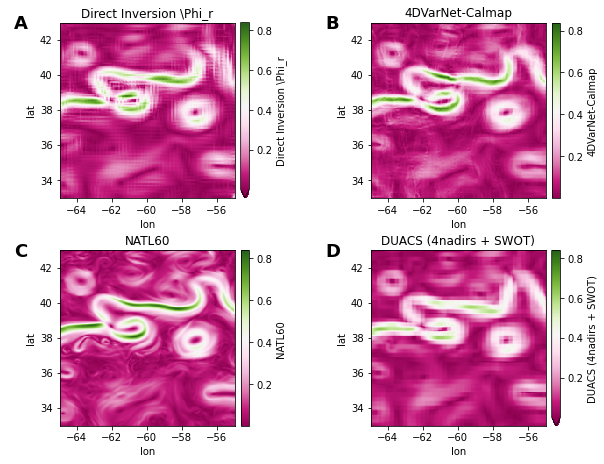
\includegraphics[width=8.0cm]{figs/new_grid_grad_w_phi}}
%  \vspace{2.0cm}
	\caption{Magnitude of the spatial gradient of SSH  }\smallskip
\end{minipage}
\end{figure}
%

%\subsubsection{Mapping results}
In Table \ref{table:mapscores} we evaluate the benchmarked methods in terms of SSH mapping performance. We report the mean square error (MSE) of the reconstructed SSH maps w.r.t the ground truth along with the MSE for the amplitude of the spatial gradients of the SSH maps. We also assess the effective scale resolved in the reconstructed maps for each experiment as in \cite{bfn}. It comes to retrieving the smallest spatial wavelength for which the power spectral density of the true SSH is at least twice larger than that of reconstruction error. %re This is computed by considering the isotropic power spectral density average along the time dimension $iPSD$  and finding the wavelength $\lambda_{er}$ for which $iPSD(SSH)(\lambda_{er}) / iPSD(SSH - SSH^{true})(\lambdal_{er}) = 2$


%The gradient is computed using a sobel operator.

\begin{table}
{\footnotesize
\begin{tabular}{lrrr}
\toprule
metric &       mse  &  mse${}_\nabla$  & $\lambda_{er}$ \\
	&        ($1e^{-3}m^2$) &   ($1e^{-10}$) & (km) \\
\midrule
4DVarNet-Calmap${}_{\nabla}$ &  1.50 &  1.07 & 95.56 \\
\textbf{4DVarNet-Calmap}      &  \textbf{1.29} &  \textbf{1.03} & \textbf{88.21} \\
4DVarNet-Map           &  1.49 &  1.10 & 94.08 \\
DUACS 4NADIRS          &  2.53 &  1.95 & 129.26 \\
CAL + DUACS            &  2.20 &  1.74 & 125.32 \\
% swot\_oi                &  0.000902 &  0.002059 \\
% CAL + direct $\phi$    &  0.002054 &  0.004109 \\
Direct $\phi$          &  2.10 &  1.66 & 116.58 \\
CAL + Direct ViT   &  2.48 &  2.04 & 126.02 \\
\bottomrule
\end{tabular}}
\caption{Mapping scores}
\label{table:mapscores}
\end{table}

\begin{figure}[htb]
\begin{minipage}[b]{1.\linewidth}
  \centering
  \centerline{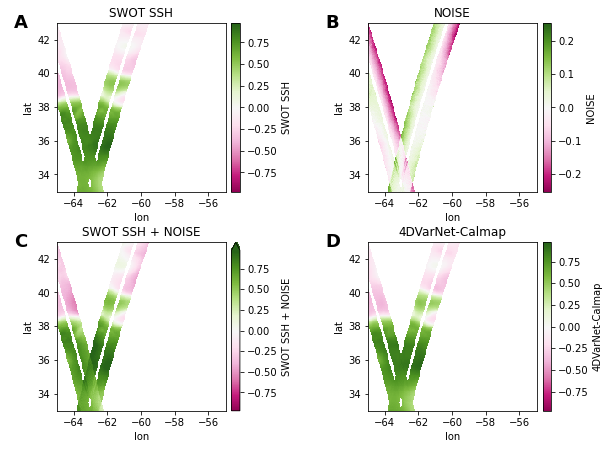
\includegraphics[width=8.0cm]{figs/square_obs_grid_sep_scale.png}}
%  \vspace{1.5cm}
	\caption{(m) A: SWOT SSH signal, B: Acquisition noise, C: Noisy Observations, D: Calibrated SSH output of 4DVarNet-Calmap}
	\smallskip
\end{minipage}
%
% \caption{SSH Fields.}
\label{fig:res}
%

\end{figure}

In table \ref{table:mapscores} 4DVarNet-Calmap models clearly outperform the operational SOTA products.
Indeed we reduce the mse up to 41.6\% (resp. 40.0\%)  w.r.t. DUACS regarding the SSH (resp. is gradient amplitude). 
.% at minimum and up to%The mse${}_\nabla$ sees an improvement of 37.0\% up to 40.0\%. 
4DVarNet-Calmap schemes resolves finer scales from 30 to 36 km. 
If we compare the different parameterizations, we can first note that even without learning jointly the calibration, the 4DVarnet-Map framework shows remarkable robustness to the acquisition noise.
We may also point out that learning jointly the calibration improves the mapping performance if more focus  during the training stage is given to the reconstruction of the SSH on the swath.
The interest of the variational framework is emphasized by  the gain we get switching from a direct architecture to the variational formulation (Direct $\phi$ vs. 4dVarNet-Map).
Training a more complex model is non trivial because of the high rate of missing data in the maps to interpolate $>90\%$, as illustrated by the relatively poor performance of the Direct Vit.


%\subsubsection{Calibration results}
In Table \ref{table:calscores}, we report the metrics of the different methods in the SWOT geometry: we interpolate again the estimated SSH on the swath. In order to handle ill-defined values that arise from this interpolation we do not consider the three outer most  across-track coordinates on each side of the nadir.
We compute the same MSE score as on the grid.
The effective resolution is computed for each pass of the satellite over the domain using the average wavenumber spectra in the along track direction. We report the mean and standard deviation of the scales resolved at each pass. The calibration metrics do benefit from the joint mapping and calibration. In order to recover finer scales of SSH signals, the focus has to be put on the reconstruction of the gradients during the training. 
\begin{table}
{\footnotesize
\begin{tabular}{lrrr}
\toprule
	{} &         mse &         mse${}_\nabla$ & $\lambda_{er}$  \\
	{} &    ($1e^{-4}$m²) &    ($1e^{-11}$) & (km) \\
\midrule
SWOT SSH + NOISE       &  51.23 &  39.16 & 51.37 ($\pm$ 56.21)\\
4DVarnet-Map           &  6.71 &  6.52 &  36.72 ($\pm$ 13.13) \\
4DVarnet-Calmap      &  \textbf{6.27} &  6.83 & 34.96 ($\pm$ 12.18)\\
\textbf{4DVarnet-Calmap}${}_{\nabla}$ &  6.79 &  \textbf{5.87} & \textbf{23.56} ($\pm$ \textbf{8.47}) \\
Direct  $\phi$        &  24.08 &  20.48 &  101.57 ($\pm$  35.23) \\
DUACS 4 NADIRS        &  27.34 &  22.50 &  97.21 ($\pm$ 85.90) \\
% Direct Inversion ViT   &  0.001284 &  0.000418 \\
\bottomrule
\end{tabular}
}
\caption{Calibration scores}
\label{table:calscores}
\end{table}

%\subsubsection{Results analysis}


\section{CONCLUSION}
We have investigated how data-driven methods can solve the joint calibration and mapping of noisy satellite altimetry data.
The proposed physics-informed learning scheme can truly benefit from the different data sources as well as prior physical knowledge. Using a simulation-based experiments, we have demonstrated its potential to outperform operational SOTA mapping methods with no requirement for a prior calibration. Future work will investigate how to transfer these results to real observation datasets.

%It significantly improves the scales resolved on the map and on the observed domain depending on the training parameterization.
% This may open the perspective of having task-oriented calibration models.
%We have shown that this method outperforms the operational SOTA mapping methods while not needing prior calibration.
%Before being considerable for operational purposes, 4DVarCalMap will need to confirm the results presented here on real satellite data and on a global scale.

% \begin{tabular}{lrrrr}
% \toprule
% {} &   spat\_res &   mean spat\_res grad &   std spat\_res &   std spat\_res grad \\
% xp\_long                &            &            &            &             \\
% \midrule
% 4DVarnet-Map           &  36.722014 &  40.928357 &  13.126934 &   15.563801 \\
% 4DVarnet-Calmap      &  34.959489 &  39.910638 &  12.182929 &   12.318272 \\
% 4DVarnet-Calmap_{\nabla} &  23.555716 &  41.928822 &   8.472936 &   18.848041 \\
% % Direct Inversion ViT   &  38.466113 &  40.921380 &  15.124034 &   17.949987 \\
% Direct  $\phi$        &  101.573017 &  101.124028 &  35.231994 &   48.753005 \\
% SWOT SSH + NOISE       &  51.372978 &  97.891729 &  56.209750 &  146.612881 \\
% \bottomrule
% \end{tabular}
% To start a new column (but not a new page) and help balance the last-page
% column length use \vfill\pagebreak.
% -------------------------------------------------------------------------
%\vfill
%\pagebreak


% References should be produced using the bibtex program from suitable
% BiBTeX files (here: strings, refs, manuals). The IEEEbib.bst bibliography
% style file from IEEE produces unsorted bibliography list.
% -------------------------------------------------------------------------
% \bibliographystyle{IEEEbib}
% \bibliography{refs}
\addcontentsline{toc}{section}{Bibliography}
\putbib[./00_JointCalMap/refs.bib]
\end{document}